\chapter{Grundlagen der Versuchsplanung}
Alle gewonnenen Beobachtungen für Y unterliegen einer Vielzahl von unterschiedlichen Einflußfaktoren. Einige davon sind bekannt (und können quantifiziert werden), andere dagegen sind unbekannt oder wirken zufällig auf die Beobachtungen $y_1,\cdots,y_n$ \\
		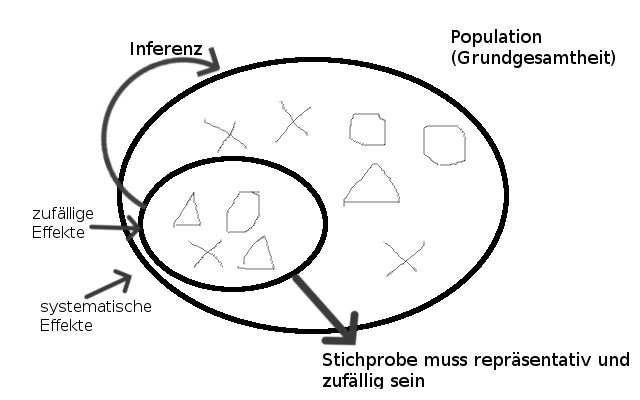
\includegraphics[scale=0.5]{VorlesungenTexDateien/images/Stichprobe}

$\Rightarrow$ alle systematischen Effekte sollten bei der Versuchsplanung mit berücksichtigt werden 
Es müssen 3 Bedingungen erfüllt sein:
\begin{enumerate}
	\item Randomisierung von Proben/Individuen zwischen den Kategorien einer kategorialen Variable
	\item Es muß auf eine ausreichende Anzahl von Replikaten geachtet werden
	\item Falls systematische Effekte bei der Versuchsdurchführung auftreten können, müssen diese bei der Verteilung der Proben auf die Prozessierungsblöcke berücksichtgt werden (\underline{Blocking})
\end{enumerate}
